\chapter{Vehicle Stuff}\label{appA}
%\addtocontents{toc}{\protect\contentsline {part}{Appendices}{}{}}

\section{Vehicle Networks}
CAN is a controller area newtwork ref to can stuff blaha..

\chapter{Rig Calculations}\label{app:rigdata}
This appendix contains calculations made for the test rig dynamics model. 

\section*{Drag force}
When calculating the drag force on the car, four terms must be known.
These are the air density, $\rho$, the drag coefficient $C_D$, the vertical area
$A$ and the current velocity of the vehicle, $v$~\cite{nakayama2002}. Air
density changes with atmospheric pressure and temperature, but is assumed to on
average be $1.205\si{kg/m^3}$ (\cite{nakayama2002} Table 2.2) in standard
atmospheric pressure, $1.013\si{kPa}$. 

Permissable estimations for the drag coefficient of a passenger car are
$0.28-0.37$~\cite{nakayama2002}. Elba is designed to be aerodynamically
efficient so a value in the lower regions is chosen, whereby $C_D = 0.30$ is
chosen.

Using geometrical methods, the area of Elba is estimated to $1\si{m^2}$.

Using these values in Equation (\ref{eq:testrig_csimple}), the combined air
resistance term of Elba is calculated to be $C_{tot} = 0.18$.

\chapter{Testrig software}
This section will contain information about the (new) software in the rig.

TODO\@:Encoder software (TLC)

\chapter{RaceCapture Pro 2 specifications}\label{app:RCP}
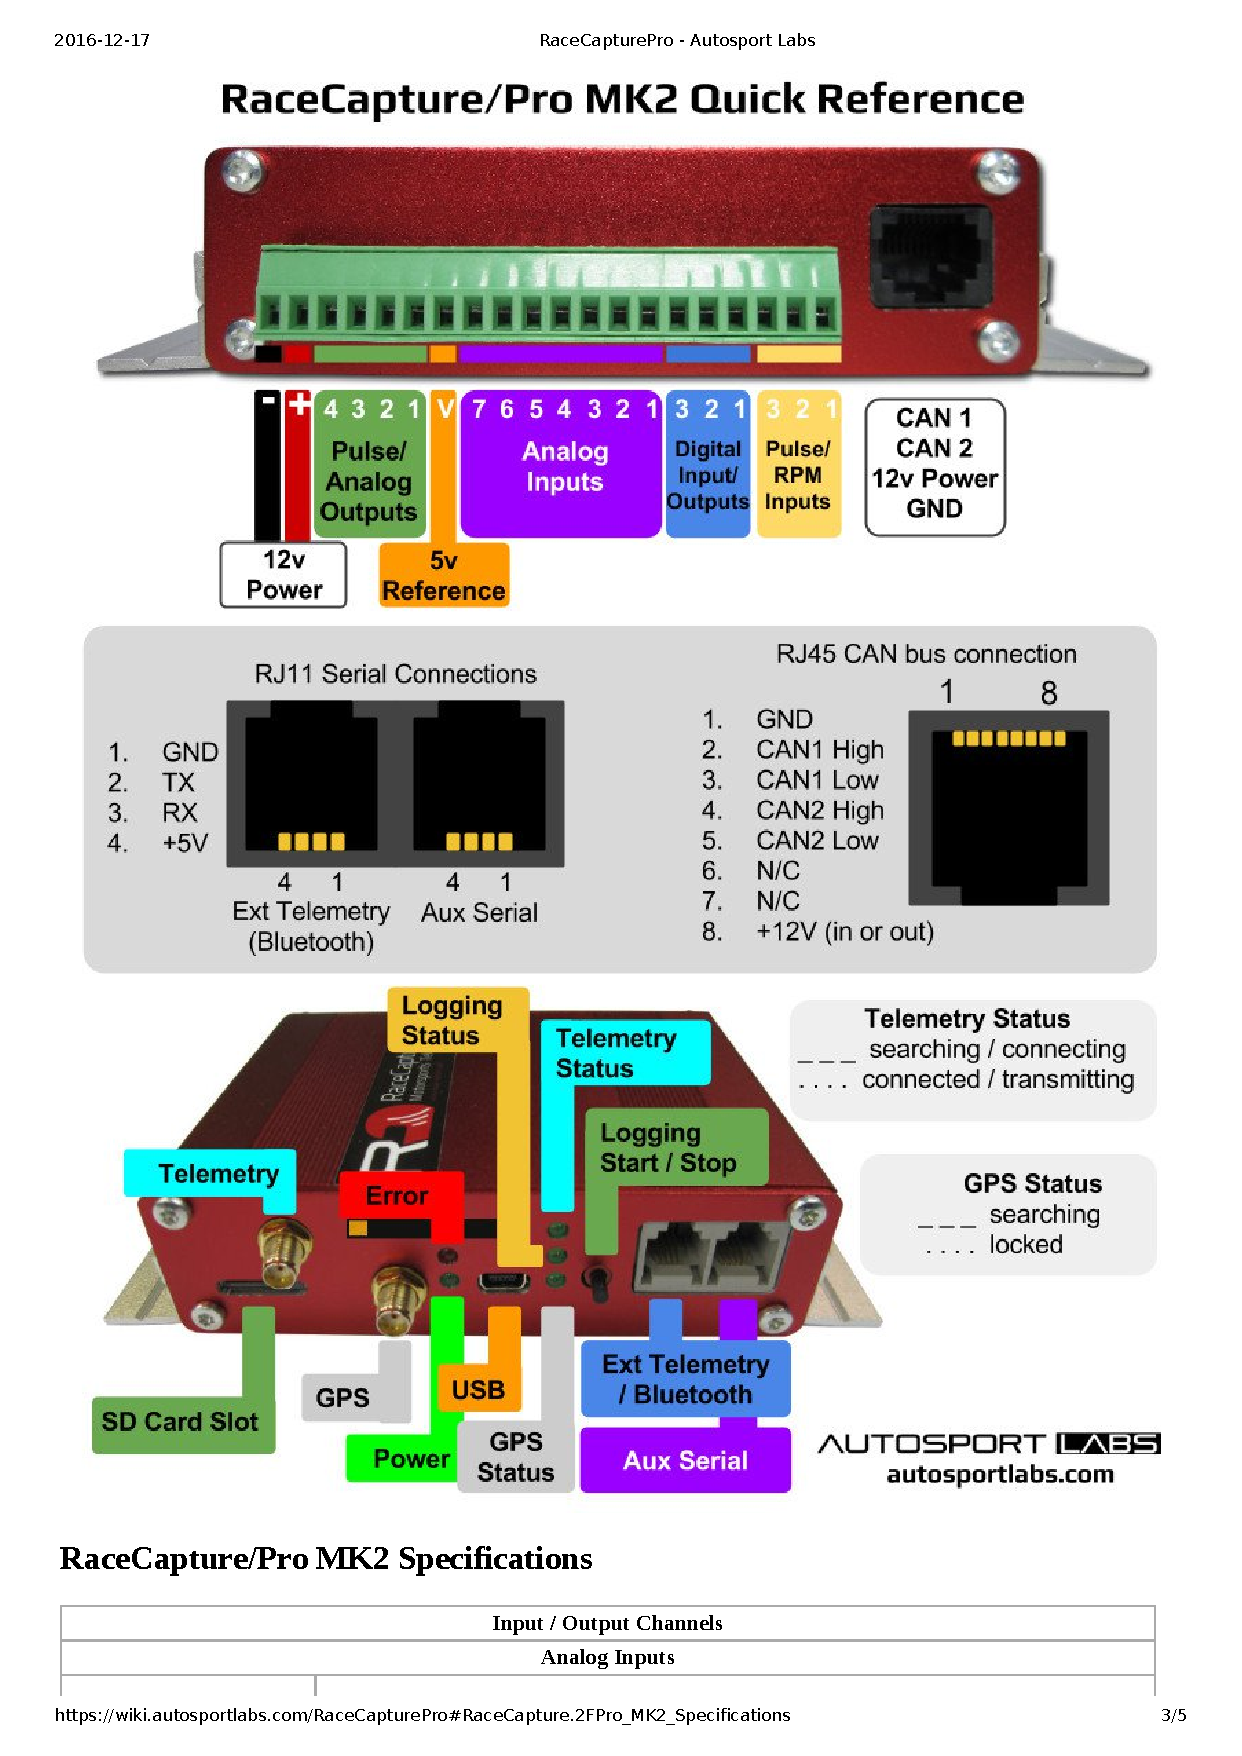
\includepdf[pages=-]{appendices/RaceCapture-Pro-MK2-quick-reference-sheet.pdf}
